% !TEX TS-program = pdflatex
\documentclass[14pt,aspectratio=169,draft]{beamer}
\usetheme{metropolis}
\metroset{progressbar=frametitle}
\usepackage{pifont}

% -------------------------------------------------------------- %
% ENCODING                                                         %
% -------------------------------------------------------------- %
\usepackage[utf8]{inputenc}
\usepackage[T1]{fontenc}
\usepackage{textcomp}

% -------------------------------------------------------------- %
% TikZ & helper libraries (ohne shadows.blur)                     %
% -------------------------------------------------------------- %
\usepackage{tikz,adjustbox}
\usetikzlibrary{positioning,arrows.meta,fit}

% -------------------------------------------------------------- %
% PGFPlots                                                           %
% -------------------------------------------------------------- %
\usepackage{pgfplots}
\pgfplotsset{
  compat=newest,
  plot coordinates/math parser=false % schneller, wenn du fixe Koordinaten hast
}

% -------------------------------------------------------------- %
% MATH & ABBREVIATIONS                                               %
% -------------------------------------------------------------- %
\usepackage{amsmath,physics,xspace}

\newcommand{\tfidf}{TF-IDF\xspace}
\newcommand{\TFIDF}{Term-Frequency-Inverse-Document-Frequency\xspace}
\newcommand{\IForest}{Isolation-Forest\xspace}
\newcommand{\RForest}{Random-Forest\xspace}
\newcommand{\LOC}{Lines of Code\xspace}

% -------------------------------------------------------------- %
% TikZ‑Stile                                                         %
% -------------------------------------------------------------- %
\tikzset{
  box/.style = {rectangle, draw, rounded corners=3pt,
                text width = 4.5cm, align = center,
                minimum height = 1.05cm,
                font = \small, fill = gray!6},
  side/.style = {box, text width = 3.8cm, fill = blue!7},
  arr/.style  = {-{Stealth[length=3mm,width=2mm]}, thick},
  lab/.style  = {font=\scriptsize, sloped, anchor=south, midway}
}

% -------------------------------------------------------------- %
% Titelinformationen                                                 %
% -------------------------------------------------------------- %
\title{Use of AI for log analysis in CI/CD pipelines}
\subtitle{Bachelor Thesis - Defence}
\author{Maid Ališi\'c}
\institute{University of Applied Sciences Upper Austria, Campus Hagenberg}
\date{23 July 2025}

% =============================================================== %
\begin{document}
% =============================================================== %

\maketitle

\section{Problem Context}
\begin{frame}{Why do we care?}
\begin{itemize}[<+->]
  \item CI/CD emits \alert{$\approx$ 10-20 GB} build, test \& deploy logs every day.
  \item Manual grepping is slow $\xrightarrow{}$ merge queue stalls, silent faults creep in.
  \item Service-level objective: deliver a verdict inside \alert{ $\leq$ 200 ms}.
  \item Logs can contain customer identifiers $\xrightarrow{}$ \textbf{no SaaS export}.
\end{itemize}
\end{frame}

\begin{frame}{Operational pain points}
\begin{enumerate}[<+->]
  \item \textbf{Context sensitivity} - same token can be harmless or fatal.
  \item \textbf{Concept drift} - every merge may rename tests or flags.
  \item \textbf{Latency pressure} - analysis must end before runner teardown.
  \item \textbf{Alert fatigue} - static regex rules explode over time.
\end{enumerate}
\end{frame}

\section{Research Questions}
\begin{frame}{Research questions (thesis)}
\begin{description}[<+->]
  \item[RQ\textsubscript{main}] How can AI improve \emph{accuracy \& explainability} of CI/CD log analysis?
  \item[RQ1] To what extent can an \textbf{LLM service} (ChatGPT API) automate log interpretation?
  \item[RQ2] How does a \textbf{local} stack (\IForest + \RForest) compare with the cloud LLM?
  \item[RQ3] Which practical hurdles arise when embedding both approaches into existing pipelines?
\end{description}
\end{frame}

\section{Method - Feature Engineering}
\begin{frame}{Vectorisation step \ding{172} – TF-IDF}
\small
\begin{enumerate}[<+->]
  \item \textbf{Normalisation:} remove timestamps, colours, IDs; lowercase.
  \item \textbf{Tokenise} + generate 1-2-grams.
  \item Compute weights  
        \[
          w_{t,d}= \mathrm{tf}_{t,d}\cdot
          \log\frac{N}{\mathrm{df}_t}\quad\text{(\TFIDF{})}
        \]
  \item Result: 50 k-dimensional sparse matrix;  
        \(\approx 100\,000\) lines /s on a single core.
\end{enumerate}

\vspace{0.5em}
\centering
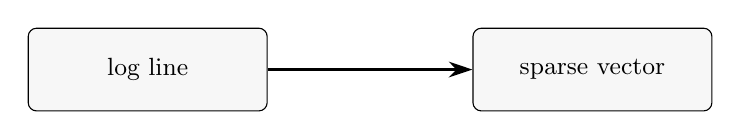
\begin{tikzpicture}[node distance=1.1cm]
  \node[box,text width=2.8cm] (txt){log line};
  \node[box,right=2.6cm of txt,text width=2.8cm] (vec){sparse vector};
  \draw[arr](txt)--(vec);
\end{tikzpicture}
\end{frame}

% --------------------------------------------------------------- %
\section{Method - Algorithm \ding{173}}
\begin{frame}{How Isolation-Forest detects outliers}
\begin{columns}
\column{0.55\linewidth}
\begin{itemize}[<+->]
  \item Randomly split feature space into binary trees.
  \item Rare / weird points are isolated \emph{early}.  
        Path length \(h(x)\) $\rightarrow$ anomaly score  
        \(s(x)=2^{-h(x)/c(n)}\).
  \item CPU-friendly: \(30 \mu\text{s}\) per line, no GPU.
\end{itemize}

\column{0.45\linewidth}
\centering
\begin{adjustbox}{max width=\linewidth}
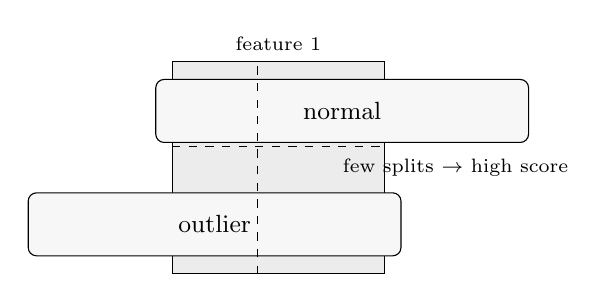
\begin{tikzpicture}[scale=.9]
  \draw[fill=gray!15] (0,0) rectangle (3,3);
  \node at (1.5,3.25) {\scriptsize feature 1};
  \node[box,minimum width=1cm,minimum height=.8cm] (p1) at (0.6,.7){outlier};
  \node[box,minimum width=1cm,minimum height=.8cm] (p2) at (2.4,2.3){normal};
  \draw[dashed] (1.2,0)--(1.2,3) (0,1.8)--(3,1.8);
  \node at (4,1.5){\scriptsize few splits $\rightarrow$ high score};
\end{tikzpicture}
\end{adjustbox}
\end{columns}
\end{frame}

\section{Method - Algorithm \ding{174}}
\begin{frame}{Why add a Random-Forest classifier?}
\begin{columns}
\column{0.53\linewidth}
\begin{enumerate}[<+->]
  \item \IForest flags \emph{that} something is odd.  
        Operators still ask \emph{why}.
  \item \RForest ensemble votes one of seven error categories.
  \item Feature importance (n-grams) enables future token-level highlights.
  \item Trains nightly in < 90 s (400 trees, depth 30).
\end{enumerate}

\column{0.47\linewidth}
\centering
\begin{adjustbox}{max width=\linewidth}
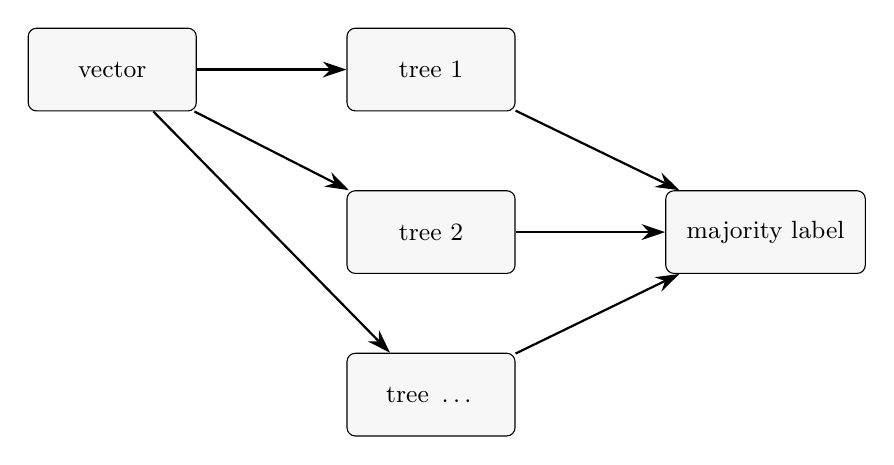
\begin{tikzpicture}[node distance=1cm]
  \node[box,text width=1.9cm] (v){vector};
  \node[box,right=1.9cm of v,text width=1.9cm] (t1){tree 1};
  \node[box,below=of t1,text width=1.9cm] (t2){tree 2};
  \node[box,below=of t2,text width=1.9cm] (t3){tree $\,\dots$};
  \node[box,right=1.9cm of t2,text width=2.3cm] (vote){majority label};
  \draw[arr](v)--(t1);
  \draw[arr](v)--(t2);
  \draw[arr](v)--(t3);
  \draw[arr](t1)--(vote);
  \draw[arr](t2)--(vote);
  \draw[arr](t3)--(vote);
\end{tikzpicture}
\end{adjustbox}
\end{columns}
\end{frame}

\section{Architecture}
\begin{frame}{End-to-end pipeline (< 40 ms inline)}
\centering
\begin{adjustbox}{max width=.9\linewidth, max height=.7\textheight}
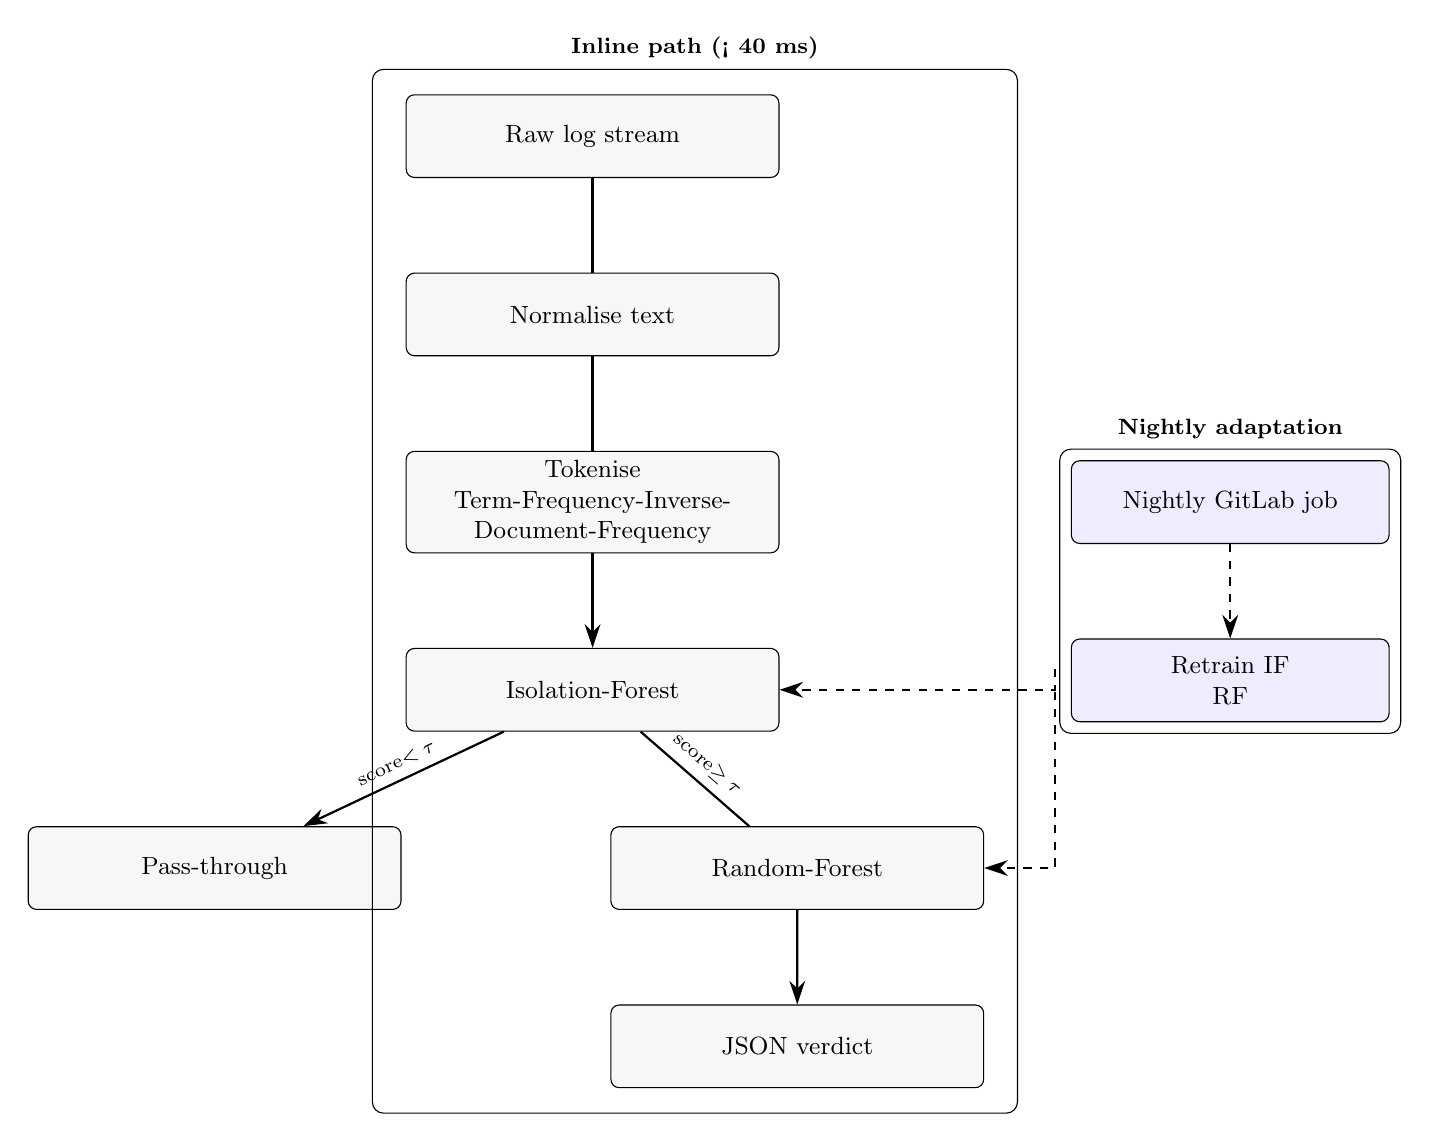
\begin{tikzpicture}[node distance=1.2cm and 1.8cm]
  \node[box] (raw){Raw log stream};
  \node[box,below=of raw] (norm){Normalise text};
  \node[box,below=of norm] (vect){Tokenise\\\TFIDF};
  \node[box,below=of vect] (ifor){\IForest};
  \node[box,below=of ifor,xshift=+2.6cm] (rfor){\RForest};
  \node[box,below=of rfor] (json){JSON verdict};
  \node[box,below=of ifor,xshift=-4.8cm] (pass){Pass-through};

  \draw[arr](raw)--(norm)--(vect)--(ifor);
  \draw[arr](ifor)--node[lab]{score$<\tau$}(pass);
  \draw[arr](ifor)--node[lab]{score$\ge\tau$}(rfor)--(json);

  \node[side,right=3.7cm of vect] (cron){Nightly GitLab job};
  \node[side,below=of cron] (train){Retrain IF\\RF};
  \draw[arr,dashed](cron)--(train);
  \draw[arr,dashed](train.west)+(-.2,.15)|-(ifor.east);
  \draw[arr,dashed](train.west)+(-.2,-.15)|-(rfor.east);

  \node[draw,rounded corners=4pt,inner xsep=12pt,inner ysep=9pt,
        fit=(raw)(json),label=above:{\footnotesize\bfseries Inline path (< 40 ms)}]{};
  \node[draw,rounded corners=4pt,inner sep=4pt,fit=(cron)(train),
        label=above:{\footnotesize\bfseries Nightly adaptation}]{};
\end{tikzpicture}
\end{adjustbox}
\end{frame}

\section{Data \& Experimental Design}
\begin{frame}{Datasets \& metrics}
\begin{columns}
\column{0.55\linewidth}
\begin{itemize}[<+->]
  \item 117 k macOS system log lines
  \item 655 k OpenSSH authentication lines
  \item 504 ground-truth anomalies
  \item Split 70 / 15 / 15 \% (train / validation / test)
  \item Metrics: Macro-F\textsubscript{1}, Area under PR curve, 99.9 \% latency
\end{itemize}

\column{0.45\linewidth}
\centering
\begin{adjustbox}{max width=\linewidth}
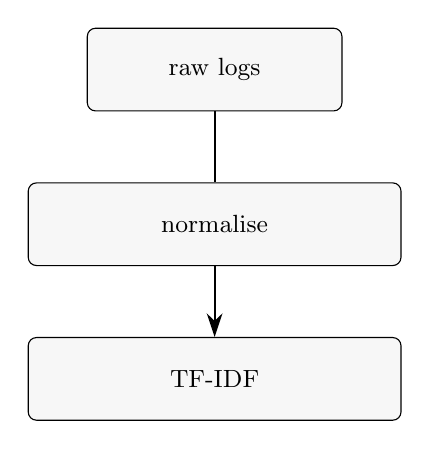
\begin{tikzpicture}[node distance=0.9cm]
\node[box,text width=3cm] (raw){raw logs};
\node[box,below=of raw] (norm){normalise};
\node[box,below=of norm] (vec){TF-IDF};
\draw[arr](raw)--(norm)--(vec);
% \node at ($(vec)!0.5!(raw)+(3.6,0)$) {\footnotesize 50 k-dim.\ sparse};
\end{tikzpicture}
\end{adjustbox}
\end{columns}
\end{frame}

\section{Results}
\begin{frame}{Headline numbers}
\begin{columns}
\column{0.55\linewidth}
\small
\begin{itemize}[<+->]
  \item Detection (\IForest): \textbf{F\textsubscript{1} = 0.89}  (AUC-PR 0.94)
  \item Diagnosis (\RForest): Macro-F\textsubscript{1} = \textbf{0.99}, MCC 0.98
  \item Latency: 37 ms (p99.9); throughput 45 k lines/s
\end{itemize}

\column{0.45\linewidth}
\centering
\begin{adjustbox}{max width=\linewidth}
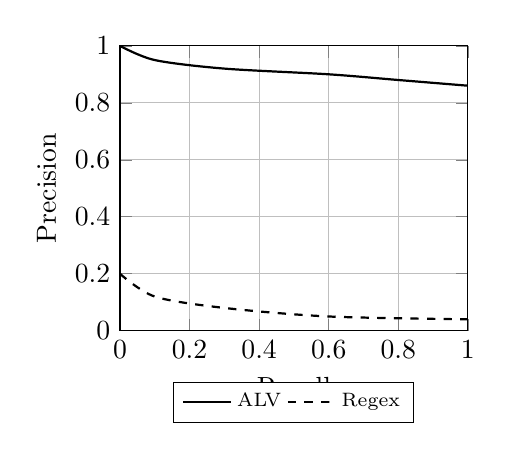
\begin{tikzpicture}
\begin{axis}[width=6cm,height=5.2cm,
             xlabel=Recall,ylabel=Precision,
             xmin=0,xmax=1,ymin=0,ymax=1,
             grid=major,legend style={font=\scriptsize,
             at={(0.5,-0.18)},anchor=north,legend columns=-1}]
  \addplot[smooth,thick] coordinates
    {(0,1) (0.1,0.95) (0.3,0.92) (0.6,0.90) (0.8,0.88) (1,0.86)};
  \addlegendentry{ALV}
  \addplot[smooth,thick,dashed] coordinates
    {(0,0.2) (0.1,0.12) (0.3,0.08) (0.6,0.05) (1,0.04)};
  \addlegendentry{Regex}
\end{axis}
\end{tikzpicture}
\end{adjustbox}
\end{columns}
\end{frame}

\section{Impact}
\begin{frame}{Organisation-level benefits}
\begin{itemize}[<+->]
  \item \alert{Minutes → Milliseconds}: failures surface during the same pipeline run.
  \item \textbf{Zero token fees}: 2300 \LOC{} + FastAPI; vendor neutral.
  \item Data never leaves the VPN - compliant with GDPR \& NDAs.
  \item Deterministic labels enable auditable root-cause trails.
\end{itemize}
\end{frame}

\section{Limitations \& Roadmap}
\begin{frame}{Limitations \& next steps}
\begin{itemize}[<+->]
  \item Only seven error classes - grow ontology as label volume rises.
  \item First Drain template pass is manual (cold-start issue).
  \item Explainability: token-level SHAP / IG still to-do.
  \item Roadmap: threshold-free Bayesian change-point, distilled LogBERT, federated retrain, SHAP highlights.
\end{itemize}
\end{frame}

\section{Wrap-up}
\begin{frame}{Take-away}
\vspace{1em}
\begin{center}
\Large
\textbf{Light-weight, on-prem ML matches AIOps SaaS}\\[0.4em]
without latency, cost or data-protection pain.
\end{center}

\vspace{1.2em}
\begin{center}
\small
Questions welcome - thank you!
\end{center}
\end{frame}

\end{document}
